\documentclass{iopjournal}
\usepackage{amsmath}
\usepackage{amssymb}
\graphicspath{{figures/}}

% Macros of the former iopart class, kept so that the text reads the same
\newcommand{\eref}[1]{(\ref{#1})}
\newcommand{\Eref}[1]{Equation~(\ref{#1})}
\newcommand{\fref}[1]{figure~\ref{#1}}
\newcommand{\Fref}[1]{Figure~\ref{#1}}
\newcommand{\tref}[1]{table~\ref{#1}}
\newcommand{\Tref}[1]{Table~\ref{#1}}
\newcommand{\rmd}{\mathrm{d}}
\newcommand{\rme}{\mathrm{e}}
\newcommand{\rhoV}{\rho V}
\newcommand{\Jone}{J^{1}}

% Running heads and article label for the submitted version
\fancyhead[L]{}
\fancyhead[R]{C Echeverr\'{\i}a-Arrondo}
\makeatletter
\renewcommand{\articletype}[1]{\noindent{\scriptsize\sf\bfseries\MakeUppercase{#1}}\par\vspace{4mm}}
\makeatother

\begin{document}

\articletype{Paper}

\title{Boost-range scaling of the fluctuations of the Benincasa--Dowker action and its consequences for Everpresent $\Lambda$}

\author{Carlos Echeverr\'{\i}a-Arrondo}

\affil{Instituto de Dise\~no para la Fabricaci\'on y Producci\'on Automatizada, MALTA Consolider Team, Universitat Polit\`ecnica de Val\`encia, 46022, Val\`encia, Spain}

\email{cecharr@idf.upv.es}

\keywords{causal sets, Benincasa--Dowker action, cosmological constant, Everpresent Lambda, fluctuations}

\begin{abstract}
Everpresent $\Lambda$ is a causal-set inspired proposal in which the
cosmological constant fluctuates as $\delta\Lambda\propto V^{-1/2}$, where $V$
is the spacetime volume of the past of the observer, an exponent inherited
from the Poisson fluctuations of the number of causal-set elements. Moradi,
Yazdi and Zilh\~ao asked whether these fluctuations could instead be sourced
by the Benincasa--Dowker (BD) action, and gave a formalism for its variance
without evaluating it. We evaluate it, analytically and with Poisson
sprinklings in four dimensions. The leading term, the Poisson noise in the
number of nearly null intervals, grows with the range of Lorentz boosts that
fits inside the region and scales exactly as $(\rhoV)^{2-2/d}$. In causal
diamonds, truncated past light cones and past cones of spatially flat FLRW
spacetimes reaching the big bang, the remaining correlation terms are a
constant fraction of this term over the simulated range ($\rhoV$ up to
$12\,800$ for the diamond and $6400$ for the cones), which bounds a residual
power law in their ratio to $|\delta|\lesssim0.1$. Extrapolating, the
asymptotic exponent is $\Delta S\propto(\rhoV)^{3/4}$, so that
$\delta\Lambda\propto V^{-1/4}$, rather than the Poisson value; the geometry
only fixes the amplitude, through a boost-range integral that we compute. For
the smeared action the same holds within a smaller range, and the physically
relevant limit of strong smearing remains an extrapolation. Reading the
action fluctuation as a fluctuation of the cosmological term, we build
zero-mean stochastic $\Lambda(t)$ histories with this scaling, the measured
temporal correlation and a free amplitude, and confront them with
Pantheon+SH0ES supernovae, DESI DR2 baryon acoustic oscillations and Planck
distance priors. None of $10^4$ histories fits the data as well as
$\Lambda$CDM ($\Delta\chi^2_{\rm min}=+124$), and the exclusion is robust
against the memory of the process and across a family of Ornstein--Uhlenbeck
dynamics.
\end{abstract}

% ---------------------------------------------------------------------------
\section{Introduction}
\label{sec:intro}

Causal set theory replaces the spacetime continuum by a locally finite
partially ordered set, whose elements are related by the causal order and
whose number counts spacetime volume~\cite{Bombelli1987,Surya2019}. A
heuristic argument by Sorkin~\cite{Sorkin1997,Sorkin2007b}, made precise in
the Everpresent $\Lambda$ model~\cite{Ahmed2004,Ahmed2013,Das2023,Das2024},
connects this discreteness with the
cosmological constant. In unimodular gravity $\Lambda$ is conjugate to the
spacetime volume $V$; if $V$ is only defined up to the Poisson fluctuation
$\delta N=\sqrt{N}$ of the number of elements, then $\Lambda$ fluctuates by
$\delta\Lambda\sim V^{-1/2}\sim H^2$. The resulting dark energy density tracks
the critical density at all epochs, which would explain why $\Omega_\Lambda$
is of order one today without fine tuning.

The exponent $-1/2$ is essential to the model. If $\delta\Lambda\propto
V^{p-1}$ with $V\sim H^{-4}$, then $\delta\Lambda/H^2\propto H^{2-4p}$, and
only $p=1/2$ gives an \emph{everpresent} $\Omega_\Lambda$. In the
phenomenological realisation of Das, Nasiri and Yazdi (Model~1 of
\cite{Das2023}), this exponent is imposed by construction: each causal-set
element contributes an independent random variable to the action term
$\Lambda V$. The authors note that ``the true causal set mechanism that gives
rise to Everpresent $\Lambda$ is not fully understood''~\cite{Das2023}.

A natural candidate for a mechanism is the causal-set action itself. The
Benincasa--Dowker (BD) action~\cite{Benincasa2010,Dowker2013} is a
discretisation of the Einstein--Hilbert action, built from counts of
intervals, whose mean reproduces the Einstein--Hilbert action in the
continuum limit, up to boundary terms~\cite{Buck2015,Dowker2025}. Moradi, Yazdi and Zilh\~ao (MYZ)~\cite{Moradi2025} developed
a formalism for the variance of this action under Poisson sprinkling and
raised the question of whether its fluctuations could be the origin of
Everpresent $\Lambda$. They expressed the variance as a set of integrals over
pairs of intervals but did not evaluate them. To our knowledge, the variance
of the BD action and its scaling with the number of elements have not been
computed since.

In this paper we compute them and follow the consequences through to
cosmological data. Our main results are:
\begin{enumerate}
\item The \emph{same-pair} term of the variance, the Poisson noise in the
number of nearly null intervals, grows exactly as $(\rhoV)^{2-2/d}$, with a
prefactor set by a boost-range integral $G$ of the region that we compute in
closed form or by quadrature and verify up to $\rhoV=10^8$
(section~\ref{sec:boost}).
\item In all the regions we simulate (causal diamonds, truncated past light
cones and past cones of flat FLRW spacetimes reaching the big bang), the
remaining correlation terms are a constant fraction of the same-pair term
within the measured range ($\rhoV\le12\,800$), for the local action and,
within a smaller range of $\epsilon\rhoV$, for the smeared one (section~\ref{sec:numerics}). The asymptotic exponent of
$\Delta S$ is therefore consistent with $3/4$ in four dimensions, not with the
Poisson value $1/2$.
\item If the action fluctuation is read as a fluctuation of the cosmological
term, $\delta\Lambda\propto V^{-1/4}$ (section~\ref{sec:lambda}). We build
stochastic $\Lambda(t)$ histories with this scaling and with the temporal
correlation that we measure along nested past cones, and confront them with
supernova, BAO and CMB data. They are excluded, as is Model~1 in our
implementation, and the exclusion is robust against the dynamical
assumptions we can vary (section~\ref{sec:data}).
\end{enumerate}
The mechanism behind the first result is well known in another guise: the
non-compactness of the Lorentz group makes the number of links, or of
intervals of any fixed small cardinality, grow without bound in a sprinkled
causal set~\cite{Bombelli2009}, and the mean abundances of small intervals in
flat regions are known exactly~\cite{Glaser2013}. The same non-compact
rapidity range biases the statistics of links~\cite{Boguna2026}. What is new
here is its role in the \emph{fluctuations} of the action: we show that it
controls their scaling, quantify the amplitude through $G$ in the regions
relevant for cosmology, and follow the consequences for a fluctuating
cosmological constant.

% ---------------------------------------------------------------------------
\section{The BD action and its variance}
\label{sec:setup}

\subsection{Sprinklings and the action}

A Poisson sprinkling of density $\rho$ into a region $M$ of a $d$-dimensional
Lorentzian manifold produces a causal set whose number of elements $N$ is a
Poisson variable with mean $\rhoV$, $V={\rm vol}(M)$. For a related pair
$y\prec x$ let $n(y,x)$ be the number of elements strictly between them, and
let $N_k$ be the number of pairs with $n=k$. We use the BD action in the form
of a sum over related pairs,
\begin{equation}
S=a_N N+\sum_{y\prec x} f\big(n(y,x)\big)\,,
\label{eq:action}
\end{equation}
which is the form analysed by MYZ~\cite{Moradi2025}. For the \emph{local}
action, $f(n)=a_n$ for $n<n_d$ and $f=0$ otherwise, with
\begin{equation}
d=2:\quad (a_N;a_0,a_1,a_2)=(1;-2,4,-2),\qquad
d=4:\quad (a_N;a_0,\dots,a_3)=\frac{4}{\sqrt6}(1;-1,9,-16,8),
\label{eq:coeffs}
\end{equation}
In four dimensions these are the coefficients of~\cite{Benincasa2010}, normalised
so that the mean action tends to $\frac{1}{2\ell^2}\int R\,\rmd V$ (plus
boundary terms~\cite{Buck2015,Dowker2025}), with $\ell=\rho^{-1/4}$; MYZ use a
different global constant. In two dimensions they are those
of~\cite{Benincasa2011}, for which the mean action of a flat causal diamond
tends to $1$, its Euler characteristic. The \emph{smeared} action of
Sorkin~\cite{Sorkin2007} and Dowker and Glaser~\cite{Dowker2013} introduces a
non-locality parameter $\epsilon\in(0,1]$, with $\epsilon=(\ell/\ell_k)^d$
for a non-locality length $\ell_k$. It has the same form~\eref{eq:action}
with
\begin{equation}
a_N=\epsilon^{2/d}a_N^{(1)},\qquad
f_\epsilon(n)=\epsilon^{1+2/d}\sum_{k<n_d}a_k^{(1)}
{n\choose k}\epsilon^k(1-\epsilon)^{n-k},
\label{eq:smeared}
\end{equation}
where $a^{(1)}$ are the local coefficients~\eref{eq:coeffs}; the overall
factor $\epsilon^{2/d}$ comes from $\ell_\epsilon^2=\ell^2/\epsilon^{2/d}$, and
the additional $\epsilon$ in $f_\epsilon$ from the normalisation of the smeared
operator~\cite{Dowker2013}. For $\epsilon=1$ the local action is recovered. The
binomial weight is the probability that a pair with $n$ elements in between
keeps exactly $k$ of them after thinning each with probability $\epsilon$, so
the smeared action can be written with ``thinned'' abundances
$\tilde N_k=\sum_{y\prec x}{n\choose k}\epsilon^k(1-\epsilon)^{n-k}$, and the
MYZ formalism applies to them with minor modifications
(appendix~\ref{app:estimators}).

\subsection{Means and the Mecke formula}

All the mean values we need follow from the Mecke formula for Poisson
processes~\cite{LastPenrose2017}. For any function $h$,
\begin{equation}
\Big\langle\sum_{y\prec x}h\big(n(y,x)\big)\Big\rangle
=\rho^2\int_M\rmd V_x\int_{M\cap J^-(x)}\rmd V_y\;
\mathbb{E}\,h\big(\mathrm{Poisson}(\rho\,{\rm vol}\,I(y,x))\big),
\label{eq:mecke}
\end{equation}
where $I(y,x)$ is the causal interval. In a flat causal diamond the inner
integral depends on $x$ only through the volume of its past within the
diamond, and~\eref{eq:mecke} reduces to two nested one-dimensional
quadratures. We also need the covariance of $N$ with the
pair sum $F=\sum_{y\prec x}f(n)$. Differentiating~\eref{eq:mecke} with respect
to the intensity gives (appendix~\ref{app:mecke})
\begin{equation}
{\rm Cov}(N,F)=\rho\,\frac{\rmd\langle F\rangle}{\rmd\rho}\,,
\label{eq:covNF}
\end{equation}
which for the local action reduces to the identity
${\rm Cov}(N,N_k)=(k+2)L_k-(k+1)L_{k+1}$ of MYZ, with $L_k=\langle N_k\rangle$.

\subsection{The MYZ decomposition}

The variance of~\eref{eq:action} is
\begin{equation}
(\Delta S)^2=a_N^2\,\rhoV+2a_N\,{\rm Cov}(N,F)+{\rm Var}(F)\,,
\label{eq:var}
\end{equation}
and MYZ decompose ${\rm Var}(F)$ according to how the two pairs
$(y_1,x_1)$, $(y_2,x_2)$ in $F^2$ share their endpoints:
\begin{equation}
{\rm Var}(F)=\Jone+J^2+J^3+2J^4+J^6_{\rm c}\,.
\label{eq:myz}
\end{equation}
Here $\Jone=\langle\sum_{y\prec x}f(n)^2\rangle$ is the \emph{same-pair} term;
$J^2$ and $J^3$ collect distinct pairs sharing their past or future endpoint;
$J^4$ collects chains $y_1\prec x_1=y_2\prec x_2$; and $J^6_{\rm c}$ is the
connected part of the contribution of pairs with four distinct endpoints,
which is non-zero only when the two intervals overlap. MYZ write all terms as
integrals over configurations of points, with the joint distribution of the
two interval cardinalities given by the volume of the intersection of the two
intervals.

We evaluated the MYZ integrals by Monte Carlo with an importance sampler
adapted to nearly null intervals. In four dimensions the intersection volume
of two causal intervals has no closed form; we computed it by quadrature,
using Green's theorem for the intersection of discs at fixed time and fixed
coordinate along one axis. In two dimensions the prediction agrees with
direct sprinklings at five densities $\rhoV=25$--$400$ ($|z|\le1.56$, 4000
sprinklings each) and, for the smeared action with $\epsilon=0.5,0.25$, at ten
more points ($|z|\le1.72$). In four dimensions the agreement holds for
$\rhoV=25,50,100$, but the Monte Carlo error grows quickly with density
(23\% at $\rhoV=100$). This makes the full MYZ integrals impractical as a
scaling tool, and in the rest of the paper we follow a different strategy:
we compute the terms that dominate asymptotically \emph{exactly}, and we
measure the remaining terms on sprinklings.

% ---------------------------------------------------------------------------
\section{The same-pair term and the boost range}
\label{sec:boost}

Consider a nearly null pair, with small proper time $\tau$ between its
endpoints. Its interval has volume $c_d\tau^d$ ($c_4=\pi/24$), so its
cardinality is a Poisson variable of mean $\mu=\rho c_d\tau^d$ that stays of
order one however large the region is. What grows with the size $L$ of the
region is the number of such pairs. Writing
$y=x-\tau(\cosh\chi,\sinh\chi\,\hat{\boldsymbol n})$, the measure of the past
hyperboloid is $\tau^{d-1}\sinh^{d-2}\chi\,\rmd\tau\,\rmd\chi\,\rmd\Omega$,
and the pair fits inside the region as long as its rapidity satisfies
$\tau\rme^\chi/2\lesssim\ell(x,\hat{\boldsymbol n})$, where
$\ell(x,\hat{\boldsymbol n})$ is the extent, in time, of the past null ray
from $x$ in the direction $\hat{\boldsymbol n}$ that remains inside the
region. The rapidity integral then gives a factor $(\ell/\tau)^{d-2}$, which
is the volume of the available range of boosts. Inserting this
in~\eref{eq:mecke} and changing variables to $\mu$ gives, for $d=4$,
\begin{equation}
\Big\langle\sum_{y\prec x}h(n)\Big\rangle\simeq(\rhoV)^{3/2}\,
\frac{G/V^{3/2}}{8\sqrt{c_4}}\,\sum_{n\ge0}h(n)\,\frac{\Gamma(n+\frac12)}{n!}\,,
\qquad
G=\int_M\rmd V_x\int_{S^2}\rmd\Omega\;\ell(x,\hat{\boldsymbol n})^2\,,
\label{eq:asym4}
\end{equation}
and in general dimension the exponent is $2-2/d$, with a weight
$\Gamma(n+2/d)/n!$. Two special cases matter.

\paragraph{Two dimensions.} For $d=2$ the boost volume is
$\ln(\ell/\tau)$ and the weight is $\Gamma(n+1)/n!=1$, so that
$\langle\sum h\rangle=\rhoV\ln(\rhoV)\sum_n h(n)+O(\rhoV)$. The variance is
Poissonian up to a logarithm, $(\Delta S)^2\simeq b\,\rhoV\ln\rhoV$ with
$b=\sum_n f(n)^2$ ($b=24$ for the local action).

\paragraph{The cross term.} For $h(n)=f(n)$ the leading term
of~\eref{eq:asym4} vanishes. For the local action in $d=4$,
$\sum_k a_k\Gamma(k+\frac12)/(k!\sqrt\pi)\propto-1+\frac92-6+\frac52=0$. This is
the same cancellation that makes the mean action finite in flat space, and
by~\eref{eq:covNF} it implies that ${\rm Cov}(N,F)$ grows only like $\rhoV$.

\medskip
Therefore, if the correlation terms in~\eref{eq:myz} do not grow faster than
$\Jone$, the variance is dominated by
\begin{equation}
\Jone\propto(\rhoV)^{2-2/d}\sum_n f(n)^2\,\frac{\Gamma(n+2/d)}{n!}
\quad\Longrightarrow\quad
\Delta S\propto(\rhoV)^{1-1/d},
\label{eq:pexp}
\end{equation}
that is, $\Delta S\propto(\rhoV)^{3/4}$ in four dimensions. The region enters
only through $G$, the integrated squared length of the past null rays: the
boost range available to nearly null intervals. The exponent is a direct
consequence of Lorentz invariance together with a cut-off set by the size of
the region, the same non-compactness that makes the number of links unbounded
in a sprinkling~\cite{Bombelli2009}; it cannot be changed by a finite
rescaling of the density.

\paragraph{Why the correlation terms should follow $\Jone$.} We have no proof
that the other terms in~\eref{eq:myz} grow no faster than $\Jone$, but there
are two heuristic reasons to expect it. First, $J^2$, $J^3$ and $J^4$ are
sums of products of the row and column sums of the matrix of pair weights
(appendix~\ref{app:estimators}), e.g.\ $\sum_x f(y,x)$ for a fixed $y$. The
boost-enhanced part of such a sum is proportional to
$\sum_nf(n)\Gamma(n+\frac12)/n!$, which vanishes by the cancellation just
described, so these terms cannot acquire a second factor of the boost range.
Second, $J^6_{\rm c}$ only receives contributions from pairs of intervals
that overlap. Two nearly null intervals overlap appreciably only if they lie
along nearly the same null direction with comparable rapidity, so for each
interval the measure of correlated partners is finite, and $J^6_{\rm c}$
inherits the boost range once, like $\Jone$. In two dimensions this is
borne out: the connected term grows with the same logarithm as $\Jone$. The
numerical tests of the next section probe this expectation directly.

The approach to the asymptotic regime is slow. The exact $\Jone$ of the local
action in the four-dimensional diamond, computed from~\eref{eq:mecke} without
Monte Carlo, has a local exponent $\frac12\,\rmd\ln\Jone/\rmd\ln\rhoV$ that
decreases from $1.26$ at $\rhoV\approx35$ to $0.96$ at $\rhoV\approx570$,
$0.88$ at $\rhoV\approx2300$ and $0.77$ at $\rhoV\approx3\times10^5$.
Exponents measured at small densities, such as the $\Delta S\propto
(\rhoV)^{1.2}$ we find for $\rhoV\le100$, are therefore pre-asymptotic.

% ---------------------------------------------------------------------------
\section{Numerical tests}
\label{sec:numerics}

\subsection{Method}

For each region we compute $\Jone$, $\langle F\rangle$ and ${\rm Cov}(N,F)$
exactly from~\eref{eq:mecke} and~\eref{eq:covNF}, measure the total variance
on independent Poisson sprinklings, and define the correlation
\emph{remainder}
\begin{equation}
r=\frac{{\rm Var}(F)-\Jone}{\Jone}
=\frac{J^2+J^3+2J^4+J^6_{\rm c}}{\Jone}\,,
\label{eq:rest}
\end{equation}
the relative size of all correlation terms. The asymptotic
exponent~\eref{eq:pexp} holds if $r$ tends to a constant. Our criterion is
that the slope of a weighted linear fit of $r$ against $\ln\rhoV$ be
compatible with zero at $4\sigma$. It was fixed before the corresponding
simulations, except for the causal diamond, where it was fixed after a first
set of five densities and before the larger ones. The point at
$\rhoV=12\,800$, the FLRW cones at $\rhoV=6400$ and the tests marked as
additional below were added, with their criteria fixed in advance, after an
independent review of a first draft. A slope compatible with zero is a weak
statement on its own, so we also quote the bound it implies on a residual
power law, $r\propto(\rhoV)^\delta$: to first order the slope equals
$\delta\,\bar r$. Such a law would change the asymptotic exponent to
$p=3/4+\delta/2$ once the correlations dominate. Each
sprinkling is an exact, independent sample of the ensemble, so no
thermalisation is involved. The statistical error of a variance estimated from
$M$ sprinklings is ${\rm std}(d^2)/\sqrt M$, with $d=S-\bar S$.

\subsection{Causal diamond}

\Fref{fig:diamond} shows the four-dimensional diamond with the local action,
for $\rhoV=25$ to $6400$ (500 to 6000 sprinklings per density). The total
variance follows the exact $\Jone$ with a constant offset, and the local
exponent of the total variance decreases with $\rhoV$ in step with that of
$\Jone$, from $1.24\pm0.04$ to $0.72\pm0.05$; on these sprinklings alone,
$r=0.317\pm0.014$ with slope $+0.006\pm0.009$. As an additional test we
combined them with the independent sprinklings of the smeared-action runs
below (at $\epsilon=1$, $\rhoV=400$--$6400$) and with 500 new sprinklings at
$\rhoV=12\,800$. The remainder at the largest density is $r=0.38\pm0.10$,
compatible with the earlier mean ($0.6\sigma$), and over the whole range
$r=0.324\pm0.012$, i.e.\ $(\Delta S)^2\simeq1.32\,\Jone$, with slope
$+0.007\pm0.008$ ($1.0\sigma$, $\chi^2=12.4$ for 8 degrees of freedom;
\fref{fig:diamond}(c)). The implied bound on a residual power law is
$-0.02<\delta<0.07$ at $2\sigma$ ($-0.07<\delta<0.12$ at $4\sigma$), i.e.\
$p\le0.78$ ($0.81$). An exponent as low as the Poisson value would require
$r\to-1$, correlations that cancel $\Jone$; we see no trend in that direction.

\begin{figure}
\centering
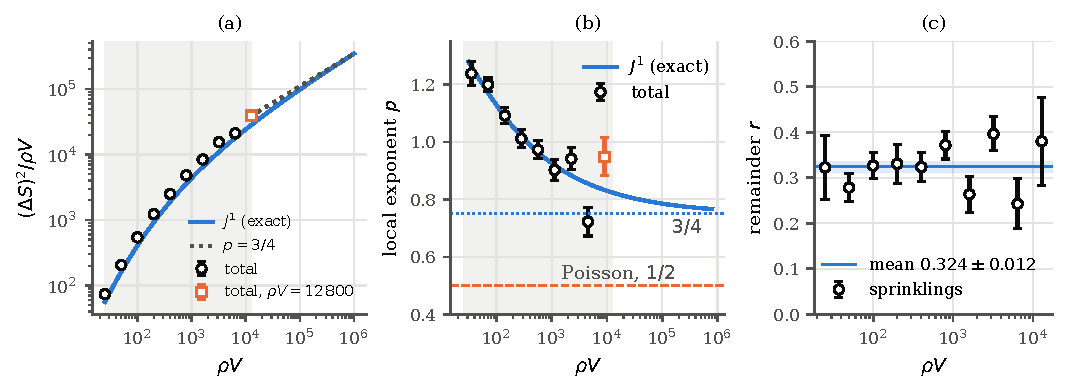
\includegraphics[width=\textwidth]{fig_diamond}
\caption{Local BD action in a four-dimensional causal diamond. (a) Total
variance per element from sprinklings (points) and the exact same-pair term
$\Jone$ (line); the dotted line has the asymptotic slope of $\Jone$, $p=3/4$.
(b) Local exponent of $\Delta S\propto(\rhoV)^p$ for $\Jone$ (line, exact)
and for the total variance (points). The total follows $\Jone$ towards
$0.75$; the Poisson value $0.5$ is not approached. (c) Remainder
$r=({\rm Var}\,F-\Jone)/\Jone$ combining all independent sprinklings,
including $\rhoV=12\,800$; the band is the weighted mean. The shading in (a)
and (b) marks the simulated range; beyond it only $\Jone$ is computed.}
\label{fig:diamond}
\end{figure}

In two dimensions (diamond, $\rhoV$ up to $12\,800$) the logarithmic law of
section~\ref{sec:boost} holds: the slope of $(\Delta S)^2/\rhoV$ against
$\ln\rhoV$ is $24.43\pm0.24$, against $b=24$ from $\Jone$ alone. Binning the
pairs that contribute to $\sum f^2$ by their rapidity
$\eta=\frac12\ln(\Delta u/\Delta v)$ gives a plateau for $|\eta|\lesssim3$,
cut off at $|\eta|\approx\frac12\ln\rhoV$: every unit of rapidity contributes
the same, which identifies the logarithm with the boost range rather than with
the boundary.

\subsection{Past light cones and FLRW}

Everpresent $\Lambda$ involves the causal past of an observer, not a diamond.
We therefore repeated the analysis for the truncated past light cone
$J^-(q)\cap\{t\ge0\}$ in Minkowski spacetime and for the past light cone of an
observer in a spatially flat FLRW spacetime, $\rmd s^2=a(\eta)^2(-\rmd\eta^2
+\rmd\boldsymbol x^2)$, reaching the big bang at $\eta=0$. We take
$a=\eta^\alpha$ with $\alpha=1$ (radiation) and $\alpha=2$ (matter). In FLRW
the interval volumes are computed exactly: at fixed $\eta$ the section of a
causal interval is a lens (the intersection of two balls), and the integral
over $\eta$ is done exactly by Gauss--Legendre quadrature in each polynomial
piece. The boost-range integral of~\eref{eq:asym4} becomes
\begin{equation}
G=\int\rmd V_x\int\rmd\Omega\int_0^{\eta_x}
\frac{2\lambda\,a(\eta_x-\lambda)^4}{\sqrt{w}}\,\rmd\lambda,\qquad
w=\frac{6}{\lambda^3}\int_0^\lambda a(\eta_y+s)^4\,s(\lambda-s)\,\rmd s,
\label{eq:Gflrw}
\end{equation}
where $\lambda$ is the conformal extent of a nearly null interval along the
null ray and $w$ is the average of $a^4$ over it, weighted by the profile
$s(\lambda-s)$ of a thin four-dimensional diamond. For $a=1$ it reduces to the
Minkowski cone.

\begin{table}
\caption{\label{tab:regions}Region dependence of the fluctuations of the
local BD action in four dimensions. $G/V^{3/2}$ is the boost-range
integral~\eref{eq:asym4}; the asymptotic ratio $\langle N_k\rangle/$(prediction)
is evaluated with the exact means at $\rhoV=10^8$ for $k=0,\dots,3$. The
remainder $r$ is the weighted mean over the simulated densities, and the slope is that
of $r$ against $\ln\rhoV$.}
\centering
\begin{tabular}{@{}lccccc}
\hline
Region & $G/V^{3/2}$ & ratio at $10^8$ & simulated $\rhoV$ & $r$ & slope of $r$\\
\hline
Diamond & $1.4472\pm0.0005$ & $0.995$--$0.987$ & $25$--$12\,800$ & $0.324\pm0.012$ & $+0.007\pm0.008$\\
Minkowski cone & $0.8187$ & $0.992$--$0.978$ & $25$--$6400$ & $0.342\pm0.017$ & $-0.001\pm0.011$\\
FLRW, $\alpha=1$ & $1.3145$ & $0.995$--$0.986$ & $25$--$6400$ & $0.346\pm0.016$ & $+0.002\pm0.010$\\
FLRW, $\alpha=2$ & $1.4194$ & $0.997$--$0.981$ & $25$--$6400$ & $0.319\pm0.015$ & $-0.004\pm0.010$\\
\hline
\end{tabular}
\end{table}

\Tref{tab:regions} summarises the results. In all regions the exact means
converge to the asymptotic form~\eref{eq:asym4}, with deviations below
$2.2\%$ at $\rhoV=10^8$ that decrease monotonically with density. For
instance, the ratio of $\Jone$ in the cone and in the diamond rises from
$0.516$ at $\rhoV=1.5\times10^5$ to $0.562$ at $10^8$, towards the predicted
$0.8187/1.4472=0.566$. The remainder is a constant fraction of $\Jone$ in all four
regions, with values between $0.32$ and $0.35$; its slope against $\ln\rhoV$
is compatible with zero in all cases (largest deviation $1.0\sigma$). The
FLRW points at $\rhoV=6400$, an additional test, give $r=0.28\pm0.08$
($\alpha=1$) and $0.37\pm0.09$ ($\alpha=2$), within $0.8\sigma$ of the earlier
means. The two
dimensional analogues behave in the same way: in the Minkowski cone and in
FLRW cones with $\alpha=1,2$ the coefficient of $\rhoV\ln\rhoV$ is
$24.09\pm0.19$, $24.26\pm0.19$ and $24.78\pm0.24$. The big bang, where
$a\to0$, does not change the scaling. The exponent is universal, and the
geometry only sets the amplitude through $G$.

\subsection{Smeared action}

The smeared action is designed to suppress fluctuations, and it is the
version that can give a phenomenologically relevant amplitude
(section~\ref{sec:lambda}). For fixed $\epsilon$ the argument of
section~\ref{sec:boost} applies unchanged, with
$\Jone_\epsilon\propto(\rhoV)^{3/2}\sum_nf_\epsilon(n)^2\Gamma(n+\frac12)/n!$,
and $\Jone_\epsilon$ is again computed exactly from~\eref{eq:mecke}. Whether
the correlation terms remain proportional to it is less clear, because the
smeared action receives contributions from intervals with up to
$\sim1/\epsilon$ elements, so the asymptotic regime requires
$\epsilon\rhoV\gg1$.

We sprinkled the four-dimensional diamond at $\rhoV=400$--$6400$ (2000 to 500
sprinklings per density) and analysed the same sprinklings with
$\epsilon=1,0.5,0.2,0.1$. The exact means and covariances~\eref{eq:covNF}
agree with the simulation in all 40 comparisons ($|z|\le2.35$), and
$\epsilon=1$ reproduces the local result, $r=0.345\pm0.025$.

Our pre-registered criterion for the smeared action was formulated for the
remainder \emph{after} subtracting the part of $F$ linear in $N$ (below),
$r_\perp=r-\rhoV g^2/\Jone$. It was met for $\epsilon=0.5$ (slope
$0.9\sigma$) but failed for $\epsilon=0.2$ and $0.1$, where $r_\perp$ grows
with $\ln\rhoV$ at $4.1\sigma$ and $6.7\sigma$. The analysis that follows,
which explains this failure, was designed after seeing it.

For $\epsilon\le0.2$ two contributions of different origin compete at these
densities. The part of $F$ that is linear in $N$, of variance
$\rhoV\,g^2$ with $g=\rmd\langle F\rangle/\rmd(\rhoV)$, is Poissonian, so it
decays relative to $\Jone$ as $(\rhoV)^{-1/2}$; for $\epsilon=0.1$ it falls
from $2.75\,\Jone$ at $\rhoV=400$ to $0.55\,\Jone$ at $6400$. To separate the
contributions we measured every MYZ term directly on each sprinkling, using
estimators built from the matrix $f(y,x)$ of pair weights and its row and
column sums (appendix~\ref{app:estimators}). The generic MYZ integrator is not usable
in this regime: at $\rhoV=6400$ its error on $J^6_{\rm c}$ was about ten times
the signal even with $4\times10^5$ samples.

\begin{figure}
\centering
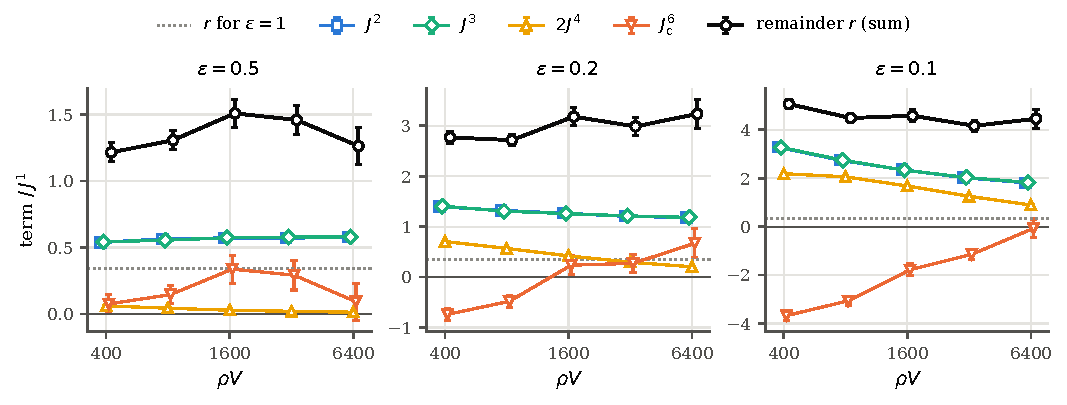
\includegraphics[width=\textwidth]{fig_smeared}
\caption{Decomposition of the correlation terms of the smeared BD action in a
four-dimensional diamond, relative to the exact same-pair term $\Jone$, for
three values of the non-locality parameter. The terms with a shared endpoint
($J^2$, $J^3$, $2J^4$) decrease with $\rhoV$ and the connected overlap term
$J^6_{\rm c}$ increases; their sum, the remainder $r$ (black), stays
approximately constant. Points of different terms are shifted horizontally by
a few per cent for clarity.}
\label{fig:smeared}
\end{figure}

\Fref{fig:smeared} shows the result. As a check, the estimated $\Jone$ agrees
with the exact value in all fifteen cases ($|z|\le0.86$), and at $\rhoV=400$,
$\epsilon=0.1$, the estimated $J^4=17.86\pm0.06$ agrees with the independent
MYZ Monte Carlo value $19.4\pm2.1$. For $\epsilon=0.5$
all terms are flat, with $r\simeq1.3$. For $\epsilon=0.2$ and $0.1$ the terms
with a shared endpoint, which carry the Poissonian part, decrease relative to
$\Jone$, while $J^6_{\rm c}$ increases (from $-3.7\,\Jone$ to
$-0.1\,\Jone$ for $\epsilon=0.1$). The two trends compensate: the total remainder
stays at $r\approx3.0$ ($\epsilon=0.2$) and $r\approx4.5$ ($\epsilon=0.1$), with
slopes against $\ln\rhoV$ of $+0.17\pm0.08$ and $-0.29\pm0.11$, both below
$3\sigma$. The growth of $r_\perp$ that made the pre-registered criterion
fail is therefore not a growing correlation: it is the approach of $r_\perp$
to $r$ as the subtracted Poissonian term decays.

Since this explanation was found a posteriori, we tested it as an additional
pre-registered criterion: the slope of the unprojected $r$, combining both
sets of sprinklings with the 500 new ones at $\rhoV=12\,800$ (which doubles
$\epsilon\rhoV$), must be compatible with zero at $4\sigma$. At
$\rhoV=12\,800$ we find $r=1.23\pm0.13$, $3.03\pm0.26$ and $4.38\pm0.32$ for
$\epsilon=0.5$, $0.2$ and $0.1$, and the slopes over $\rhoV=400$--$12\,800$
are $+0.02\pm0.03$ ($0.8\sigma$), $+0.11\pm0.05$ ($2.3\sigma$) and
$-0.25\pm0.07$ ($-3.7\sigma$). The criterion is met, though not by a wide
margin for $\epsilon=0.1$, where $r$ decreases slightly. A decreasing $r$
means that the correlations grow more slowly than $\Jone$, which does not
threaten the exponent; the upper bounds on $\delta$ at $2\sigma$ are $0.06$,
$0.07$ and $-0.02$.

Within the accessible range, $\epsilon\rhoV\le1280$, the smeared action thus
behaves like the local one: the variance is a roughly constant multiple of
$\Jone$, and $\Delta S\propto(\rhoV)^{3/4}$. The individual terms are still
drifting, so we cannot exclude a different behaviour for $\epsilon\to0$ at
fixed $\epsilon\rhoV$; we return to this point in
section~\ref{sec:discussion}.

% ---------------------------------------------------------------------------
\section{Consequences for a fluctuating $\Lambda$}
\label{sec:lambda}

\subsection{Amplitude}

To connect the action with $\Lambda$ we follow the logic of Everpresent
$\Lambda$. The BD action approximates the Einstein--Hilbert action,
$S_{\rm EH}/\hbar=\kappa S$ with $\kappa=\ell^2/(8\pi\ell_p^2)$ in our
normalisation, and the cosmological term is $\Lambda V/(8\pi\ell_p^2)$
\cite{Das2023}. Reading the action fluctuation in the past of the observer as a
fluctuation of the cosmological term gives
\begin{equation}
\delta\Lambda\,\ell^2=\frac{\Delta S}{\rhoV}\,,
\label{eq:dlambda}
\end{equation}
independently of $\ell_p$. Applied to the Poisson action of Model~1 this
reproduces its $\delta\Lambda=8\pi\alpha/\sqrt V$ exactly. This only checks
the normalisation $\kappa$, since Model~1 defines its fluctuating term
through the same relation; equation~\eref{eq:dlambda} itself is a working
hypothesis, not a consequence of a causal-set dynamics. Note also that we use
only the \emph{fluctuation} of the action: its mean in a region with a
boundary contains boundary and corner terms~\cite{Buck2015,Dowker2025}, which
play no role here. With the results of section~\ref{sec:numerics},
\begin{equation}
\delta\Lambda\,\ell^2=A\,(\rhoV)^{-1/4},\qquad
A^2=(1+r)\,\frac{G/V^{3/2}}{8\sqrt{c_4}}\sum_nf(n)^2\frac{\Gamma(n+\frac12)}{n!}\,.
\label{eq:amplitude}
\end{equation}
For the present past cone of a Planck 2018 $\Lambda$CDM
background~\cite{Planck2018}, $V\approx6.4\times10^{242}\,\ell_p^4$. With
the local action and $\ell=\ell_p$ this gives
$\delta\Lambda/\Lambda_{\rm obs}\sim10^{62}$; matching the observed value would
require $\ell\sim10^{27}\,$m, larger than the Hubble radius. The local action is
therefore excluded as a source.

For the smeared action we find numerically that
$\sum_nf_\epsilon(n)^2\Gamma(n+\frac12)/n!\to4.112\,\epsilon^{5/2}$ as
$\epsilon\to0$, so $A\propto\epsilon^{5/4}=(\ell/\ell_k)^5$. The observed
$\Lambda$ is obtained for $\ell_k\approx2.5\times10^{-23}\,$m with
$\ell=\ell_p$ ($\epsilon\sim10^{-49}$), or $\ell_k\approx1.2\times10^{-22}\,$m
with $\ell=\ell_{\rm cs}=7.1\,\ell_p$, the discreteness length that corresponds
to $\alpha=0.01$ in Model~1. These values use $r=0.33$; since
$\ell_k\propto(1+r)^{1/10}$, the larger $r\approx3$--$4.5$ found above for small
$\epsilon$ raises them by at most $15\%$. This is below the bound $\ell_k\lesssim10^{-19}\,$m derived from
$8\,$TeV LHC data, and inside the range, from $2\times10^{-22}$ to
$10^{-29}\,$m, that proposed optomechanical experiments could
probe~\cite{Belenchia2016}. It
requires, however, a large hierarchy $\ell_k/\ell_p\sim10^{12}$, so the
coincidence problem that Everpresent $\Lambda$ was meant to solve reappears as
a tuning of $\ell_k$. Equation~\eref{eq:amplitude} also changes the
\emph{time} dependence: since $\delta\Lambda\propto V^{-1/4}\propto H$ in
the matter era, the envelope $\delta\Lambda/3H^2$ behaves as a fluid with
$w\approx-1/2$, negligible at recombination ($\sim4\times10^{-5}$ at $z=1100$)
and growing until today, whereas for Model~1 $w\approx0$.

\subsection{Temporal correlation along the worldline}

A stochastic $\Lambda(t)$ also requires the correlation of $\Delta S$ between
the past cones of two instants of the same worldline. These cones are nested,
and since the region is causally convex every pair of the smaller cone is a
pair of the larger one with the same cardinality. A single sprinkling of the
largest cone therefore gives the action of all the nested cones. We measured it
for the local action in four dimensions, in the Minkowski cone and in the
matter-dominated FLRW cone (4000 sprinklings each, $\rhoV=200$, $500$, $1250$
and $3200$). The action is close to a random walk, with a small positive
memory: the correlation between the action and its increment is
$\kappa=0.069\pm0.015$ (weighted mean of the six pairs of adjacent cones;
no individual pair reaches $4\sigma$). We parametrise the correlation between
the actions $S_i$, $S_j$ of two nested cones, $V_i<V_j$, as
\begin{equation}
{\rm corr}(S_i,S_j)=\left(\frac{{\rm Var}\,S_i}{{\rm Var}\,S_j}\right)^{\beta/2},
\label{eq:beta}
\end{equation}
where $\beta=1$ is a random walk with independent increments, and find
$\beta=0.88$--$0.97$ over all pairs of cones. A pre-registered requirement that
$|\kappa|<0.2$ for every pair of cones failed for one non-adjacent pair in each geometry
($\kappa=0.29\pm0.12$ and $0.23\pm0.09$), a criterion that, in retrospect,
ignored their errors; it does not affect the value of $\beta$.

% ---------------------------------------------------------------------------
\section{Confronting the data}
\label{sec:data}

\subsection{Stochastic model}

We model the cosmological constant along the observer's worldline as
\begin{equation}
\Lambda(t)=\lambda\,V(t)^{-q}\,s(t),
\label{eq:model}
\end{equation}
where $V(t)$ is the volume of the causal past and $s$ is an
Ornstein--Uhlenbeck process~\cite{Uhlenbeck1930} in $\ln V$ with unit
variance and ${\rm corr}(s_1,s_2)=(V_1/V_2)^c$. Model~1 of
\cite{Das2023} corresponds to $q=c=1/2$ and $\lambda=8\pi\alpha$. The BD
action, with~\eref{eq:dlambda}, corresponds to $q=1/4$ and $c=3\beta/4$, and we
take $\beta=0.9$ from the measurement above. The background is integrated with
feedback, $(H/H_{100})^2=\omega_r a^{-4}+\omega_m a^{-3}+\Lambda/3$, with
$V$ accumulated along the way. We set $\Lambda=0$ before $z=10^4$, start the process
from zero and count realisations with $H^2<0$ as collapsed. This is the
convention that reproduces the completion fractions published for
Model~1 (10\,000, 3258 and 575 out of 10\,000 for $\alpha=0.005$, $0.01$
and $0.012$, against 9990, 3228 and 535 in~\cite{Das2023}).

We follow the per-seed method of \cite{Das2024}. Each seed fixes the random
numbers of the process, and for each seed we minimise $\chi^2$ over
$\omega_m$, the amplitude ($\alpha$ or $\lambda$) and the supernova magnitude
$M_B$. A seed is \emph{good} if $\chi^2<\chi^2_{\Lambda{\rm CDM}}+14.7$.
The margin is that implied by \cite{Das2024}, who count seeds with
$\chi^2<1500$ against their $\Lambda$CDM value of $1485.3$ for supernovae
alone. Our own supernova-only $\Lambda$CDM fit gives $1452.0$, with best-fit
parameters that agree with~\cite{Brout2022}; we could not reconstruct the
exact configuration behind $1485.3$, so we always apply the margin relative
to our own $\Lambda$CDM fit to the same data. The data are:
\begin{itemize}
\item Pantheon+SH0ES supernovae~\cite{Scolnic2022,Brout2022,Riess2022}, with
the standard cut (1657 light curves, 77 of them Cepheid calibrators) and the
full statistical and systematic covariance;
\item DESI DR2 BAO~\cite{DESI2025}: 13 measurements of $D_V/r_d$, $D_M/r_d$
and $D_H/r_d$ at 7 redshifts, with their covariance;
\item Planck 2018 distance priors~\cite{Chen2019} on $R$ and $l_A$, with
$\omega_b=0.02236$, the sound horizon integrated over each history, and
$z_*$, $z_{\rm drag}$ from the fits of \cite{HuSugiyama1996,EisensteinHu1998}
anchored to their Planck values.
\end{itemize}
The pipeline reproduces the Planck 2018 sound horizons to $0.08\%$ and $R$,
$l_A$ within $1\sigma$, and the DESI value of $\Omega_m$ from BAO alone
($0.2972$ against $0.2975\pm0.0086$). The treatment of radiation is
simplified (no massive neutrinos, fixed $\omega_r$), which induces a
systematic of order $0.1$--$0.2\%$ in $l_A$. A variant in which $l_A$ and
$r_d$ are rescaled so that the Planck best fit reproduces their published
values exactly gives the same conclusions. Distance priors assume standard
early physics. This holds for the BD model, where $\Lambda/3H^2\sim4\times10^{-5}$
at $z=1100$, but not for Model~1 ($\sim0.5$), which we therefore fit to
supernovae and BAO only.

\subsection{Results}

With supernovae alone both models produce rare histories that fit as well as
$\Lambda$CDM: $0.25\%$ of good seeds for Model~1, consistent with the $\approx
0.3\%$ of \cite{Das2024}, and $0.48\%$ for the BD action. The good BD seeds
fix $\ell_k\approx3\times10^{-23}\,$m, consistent with the value inferred from
the amplitude alone. Both, however, prefer $\Omega_m\approx0.5$.

\begin{table}[htb]
\caption{\label{tab:data}Fits of stochastic $\Lambda(t)$ histories (10\,000
seeds per row). $\Delta\chi^2$ is relative to the $\Lambda$CDM fit to the same
data ($\chi^2=1488.2$ for SN + BAO, $1504.0$ for SN + BAO + CMB). The last
column splits the $\Delta\chi^2$ of the best seed by probe. Model~1 is shown
without the CMB, for which the distance priors are not applicable to it.}
\centering
\begin{tabular}{@{}lccc}
\hline
Model & good seeds & $\Delta\chi^2_{\rm min}$ & best seed: SN / BAO / CMB\\
\hline
\multicolumn{4}{@{}l}{SN + BAO}\\
Model 1 ($q=c=\frac12$) & 0 & $+87$ & $+46$ / $+40$ / --\\
BD, $\beta=0.9$ & 0 & $+26$ & $-13$ / $+39$ / --\\
\hline
\multicolumn{4}{@{}l}{SN + BAO + CMB}\\
BD, $\beta=0.5$ & 0 & $+45$ & $+40$ / $+4$ / $+1$\\
BD, $\beta=0.88$ & 0 & $+116$ & $+47$ / $+69$ / $+0.5$\\
BD, $\beta=0.9$ & 0 & $+124$ & $+37$ / $+82$ / $+4.5$\\
BD, $\beta=0.97$ & 0 & $+135$ & $+50$ / $+79$ / $+6$\\
BD, $\beta=1$ & 0 & $+154$ & $+56$ / $+79$ / $+20$\\
\hline
\end{tabular}
\end{table}

Adding BAO changes the picture (\tref{tab:data}). Already without the CMB,
none of the $10^4$ seeds of either model is good (fraction below
$3\times10^{-4}$ at 95\% confidence): $\Delta\chi^2_{\rm min}=+87$ for
Model~1 and $+26$ for the BD action, with $\Lambda$CDM refitted to SN + BAO.
For Model~1 this agrees with the full Planck analysis of \cite{Das2024},
which found $\Delta\chi^2>150$, here by an independent route that does not
use the CMB. The best BD seed fits the supernovae better than $\Lambda$CDM
($-13$) but misses the BAO by $+39$: no history achieves simultaneously the
shape of the distance--redshift relation required by the supernovae and the
scale required by the BAO. Adding the CMB, which is applicable to the BD
model because its $\Lambda$ is negligible at recombination, raises the minimum
to $+124$ (with $\beta=0.9$), and none of the seeds that were good with
supernovae alone survives.

\begin{figure}
\centering
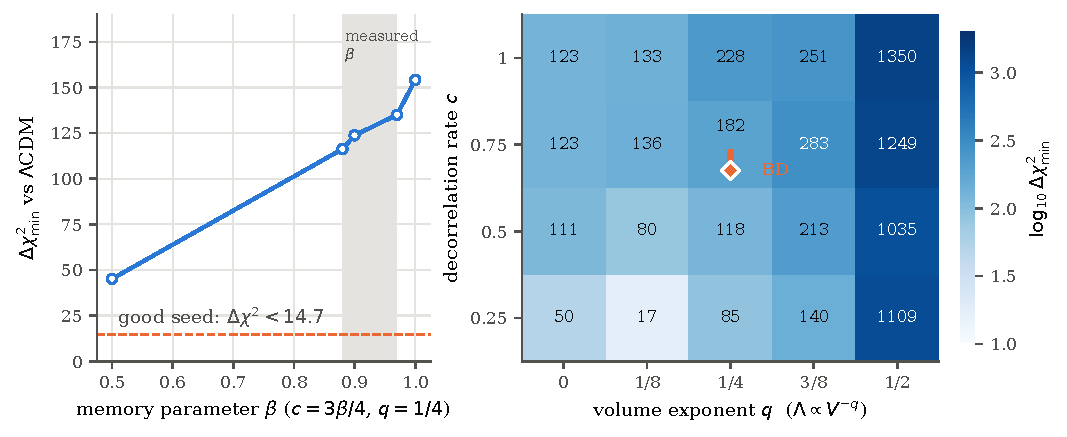
\includegraphics[width=\textwidth]{fig_data}
\caption{Robustness of the exclusion. Left: minimum $\Delta\chi^2$ with respect
to $\Lambda$CDM for the BD dynamics ($q=1/4$) as a function of the memory
parameter $\beta$ (10\,000 seeds each); the dashed line is the threshold for a
good seed and the band marks the measured range of $\beta$. Right: minimum
$\Delta\chi^2$ over the $(q,c)$ family of Ornstein--Uhlenbeck dynamics (1000
seeds per cell). Model~1 is the cell $q=c=1/2$. The diamond marks the BD
action ($q=1/4$, $c=3\beta/4$ with $\beta=0.9$) and the bar the measured range
of $\beta$. With 1000 seeds per cell the minima are somewhat higher than with
the $10^4$ seeds of the left panel (e.g.\ $+182$ at $c=0.75$ against $+154$
for $\beta=1$).}
\label{fig:data}
\end{figure}

\Fref{fig:data} tests the robustness of this conclusion. Over the measured
range of the memory parameter, $\beta=0.88$--$0.97$, the minimum
$\Delta\chi^2$ stays between $+116$ and $+135$, and even an unrealistically
long memory ($\beta=0.5$) remains above the threshold. Over the whole family
$(q,c)\in[0,\frac12]\times[\frac14,1]$ no cell has good seeds. The best cell,
$q=1/8$, $c=1/4$, reaches $+17$ with 1000 seeds; since this is close to the
threshold, we repeated it with $10^4$ seeds as an additional test, with the
same result: no good seed and $\Delta\chi^2_{\rm min}=+17.0$. The data only
tolerate a $\Lambda$ that
depends weakly on the volume and decorrelates slowly, i.e.\ one close to a
true constant. The Model~1 exponent $q=1/2$ is the worst column of the map
($\Delta\chi^2>1000$).

% ---------------------------------------------------------------------------
\section{Discussion}
\label{sec:discussion}

We have evaluated the fluctuations of the BD action that MYZ left as an open
question. The central result is structural: in $d$ dimensions the variance is
dominated by the Poisson noise in the number of nearly null intervals, whose
number is controlled by the volume of the boost group that fits inside the
region, and this gives $\Delta S\propto(\rhoV)^{1-1/d}$. Only for $d=2$ is the
exponent $1/2$, and then with a logarithm. In four dimensions the exponent is
$3/4$ in every region we tested, including the past cone of an FLRW observer
reaching the big bang, and for the local and the smeared actions. A
cosmological constant sourced by these fluctuations would scale as
$\delta\Lambda\propto V^{-1/4}$, not as the $V^{-1/2}$ of Everpresent
$\Lambda$, and a stochastic history built on this scaling does not fit
current data.

This does not refute Everpresent $\Lambda$ as such, whose original argument
relies on the Poisson fluctuation of $N$ and not on the action. It shows that
the action, the most natural dynamical quantity of the theory, does not
provide the required mechanism. The obstruction is Lorentz invariance itself:
any observable that counts intervals of fixed small volume inherits the boost
range of the region. The same non-compactness biases the statistics of links
in sprinkled causal sets~\cite{Boguna2026}. A mechanism that yields $V^{-1/2}$
would have to suppress the contribution of highly boosted intervals, for
instance through a boundary term or through a choice of frame that breaks
local Lorentz invariance.

Our conclusions have the following limitations.
\begin{enumerate}
\item \emph{Asymptotics.} The exponent $3/4$ rests on one exact ingredient
($\Jone\propto(\rhoV)^{3/2}$, verified up to $\rhoV=10^8$) and one empirical
one: that the correlations remain a constant fraction of $\Jone$. We verified
the latter up to $\rhoV=12\,800$ in the diamond and $6400$ in the past cones,
with a residual power law bounded by $\delta<0.07$ ($2\sigma$), and for the
smeared action up to $\epsilon\rhoV=1280$. The physically relevant regime,
$\rhoV\sim10^{242}$ with $\epsilon\sim10^{-49}$, is an extrapolation over
some 238 decades, which the heuristic argument of section~\ref{sec:boost}
supports but does not prove. In particular, for $\epsilon\le0.2$ the
individual MYZ terms still drift at the largest densities, and only their sum
is constant.
\item \emph{Identification.} Equation~\eref{eq:dlambda} is an assumption,
motivated by the cosmological term of the Einstein--Hilbert action and
consistent with Model~1, but not derived from a dynamics for causal sets.
\item \emph{Dynamics.} The data analysis uses a homogeneous $\Lambda(t)$ and
the Ornstein--Uhlenbeck family~\eref{eq:model}. Spatial fluctuations of
$\Lambda$ are further constrained by the isotropy of the
CMB~\cite{Barrow2007}; non-Gaussian processes or a different coupling
between the action and $\Lambda$ were not explored. The temporal memory was
measured for the local action only.
\item \emph{Statistics.} The per-seed fits use a grid search rather than the
MCMC of \cite{Das2024}, which may underestimate the fraction of good seeds;
with $\Delta\chi^2_{\rm min}=+124$ this would not change the conclusion. Our
supernova-only $\Lambda$CDM $\chi^2$ differs from that of \cite{Das2024}
(section~\ref{sec:data}); all our margins are relative to our own fits.
\end{enumerate}
Earlier cosmological tests of Everpresent $\Lambda$ are those of
\cite{Ahmed2004,Zwane2017,Das2024}; to our knowledge this is the first
confrontation of Everpresent-type dynamics with the DESI DR2 BAO data.

\ack{The numerical code, the analysis and the drafting of this manuscript were
carried out with the assistance of Claude (Anthropic), an AI model. The author
designed the project, reviewed all results and takes full responsibility for
the content.}

\data{The code that produces every number and figure of this paper, together with
its test suite (213 automated tests) and the saved intermediate results, is
publicly available at
\url{https://github.com/carlosecheverriaarrondo/Conjuntos_causales}. The
supernova and BAO data are public and are downloaded, with checksum
verification, by a script in the repository. Most tests check the code
against exact results or fresh sprinklings; some re-read the saved results of
the long runs and check the criteria quoted here. All statistical tolerances
were fixed in advance, and each group of tests was checked to fail under a deliberately
introduced error. A detailed log of every criterion, including those that
failed, is part of the repository.}

% ---------------------------------------------------------------------------
\appendix

\section{Covariance with the number of elements}
\label{app:mecke}

Let $\eta$ be a Poisson process of intensity $\rho$ on $M$ and $F(\eta)$ a
functional with finite second moment. The Mecke
equation~\cite[theorem~4.1]{LastPenrose2017} gives
$\mathbb{E}[N F]=\rho\int_M\mathbb{E}[F(\eta+\delta_x)]\,\rmd x$, while
differentiating with respect to the intensity gives
$\rho\,\rmd\mathbb{E}[F]/\rmd\rho=\rho\int_M\mathbb{E}[F(\eta+\delta_x)-
F(\eta)]\,\rmd x$. Subtracting $\mathbb{E}[N]\,\mathbb{E}[F]=\rhoV\,
\mathbb{E}[F]$ from the first expression yields~\eref{eq:covNF}. For the local
action, $F=\sum_ka_kN_k$ and $\langle N_k\rangle$ depends on $\rho$ only through
$\rhoV$, which leads to ${\rm Cov}(N,N_k)=(k+2)L_k-(k+1)L_{k+1}$. We evaluate
$\rmd\langle F\rangle/\rmd\rho$ with a central difference and checked it
against this identity (relative error below $10^{-4}$) and against sprinklings
of the smeared action.

\section{Estimators of the MYZ terms}
\label{app:estimators}

\paragraph{Smeared action.} With thinned abundances the MYZ formalism carries
over with three changes: the means become
$\langle\tilde N_k\rangle=L_k(\epsilon\rhoV)/\epsilon^2$; $\Jone$ is no longer
diagonal in $k$, because the two factors of a single pair are independent
thinnings of the same interval; and in the joint distribution of two
overlapping intervals the overlap is split into points kept by both
(probability $\epsilon^2$) and points kept by only one ($\epsilon(1-\epsilon)$
each), since thinning a Poisson process produces independent Poisson
processes.

\paragraph{Per-sprinkling estimators.} Let $f(y,x)=f(n(y,x))$ for $y\prec x$
and $0$ otherwise, with row sums $R_y=\sum_xf(y,x)$ and column sums
$C_x=\sum_yf(y,x)$. Sorting the terms of $F^2$ by shared endpoints gives,
sprinkling by sprinkling,
\begin{equation}
\sum f^2\to\Jone,\quad
\sum_yR_y^2-\sum f^2\to J^2,\quad
\sum_xC_x^2-\sum f^2\to J^3,\quad
\sum_zC_zR_z\to J^4,
\end{equation}
and $J^6_{\rm c}$ is obtained by subtracting all of them from $(F-\langle
F\rangle)^2$. The expectation of each statistic is the corresponding MYZ term,
so the estimators are unbiased up to $O(1/M)$ from the sample mean. We checked
the decomposition against an explicit enumeration of pairs of pairs.

\bibliographystyle{iopart-num}
\bibliography{refs}

\end{document}
